%!TEX root = ../report_template.tex
\paragraph{Correlation and Relationships}
The relationships can be explored by combining the datasets, plotting the interesting variables, and calculating the correlation coefficients between them. Since the student-to-teacher ratio aggregates the number of students and teachers, this section will correlate the other variable against it.

Therefore, the first  correlation exists between the average Abitur grade in Germany and the student-to-teacher ratio. Initially, the average grades across all federal states are calculated and then compared to the student-to-teacher coefficient for German grammar schools. As shown in \autoref{fig:regression-stt-grade} the relationship between both is nearly linear. In addition, the result contains neither clusters nor outliers. Hence, a smaller student-to-teacher ratio results in better grades. Additionally, the Pearson correlation value is $0.98$, indicating a strong positive correlation. This emphasizes the initial hypothesis and increases the importance of a good care factor between teachers and children.

\begin{figure}[h]
    \centering
    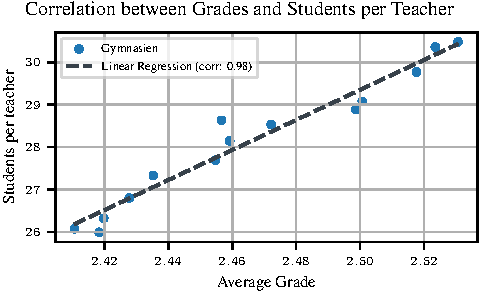
\includegraphics{fig/fig_correlation_grades_students_per_teacher.pdf}
    \caption{Linear regression on the students-to-teacher ratio by average Abitur grade. The resulting regression line (\textcolor{TUred}{\rule[-0.2ex]{0.5em}{2pt} \rule[-0.2ex]{0.5em}{2pt}}) is calculated over the aggregated average overall grammar schools (\textcolor{TUlightblue}{\tikz\draw[fill={TUlightblue}] (0,0) circle (0.25em);}) in Germany.}
    \label{fig:regression-stt-grade}
\end{figure}

As already explained, these results correspond only to grammar schools and are not necessarily representable for other schools or single federal states. Thus, the student-to-teacher ratio is also compared to the repeaters and the budgets per child in each federal state. Therefore, their Pearson correlation coefficients are calculated for each federal state across all years. 

\autoref{fig:heatmap_correlation_students_per_teacher_repeaters_budget} presents a visualization of the Pearson correlation coefficients, analyzing the relationship between the number of children per teacher and the average number of repeaters, as well as the educational budget per child. To visually represent the data across various federal states, a heatmap is generated. Therefore, the Pearson correlation coefficients for each state is normalized to the used color map scale. Consequently, each state is assigned a color representing the correlation coefficient. It is evident that there exists a strong positive correlation between the student-to-teacher ratio and the rate of repeaters in the most new federal states, while the correlation in the new federal states is significantly weaker. Moreover the correlation between the student-to-teacher ratio and the inflation adjusted budget per child tends to be positive for the new federal states and negative for the old federal states.

\begin{figure}[h]
    \centering
    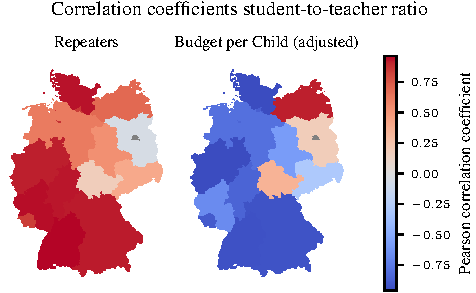
\includegraphics{fig/fig_heatmap_correlation_students_per_teacher_repeaters_budget.pdf}
    \caption{Pearson correlation coefficients between the student-to-teacher ratio and the relative repeater count (left) and the inflation-adjusted average budget per child (right). \textcolor{red}{Red} indicates positive, \textcolor{gray}{gray} neutral, and \textcolor{blue}{blue} negative correlations between the variables.}
    \label{fig:heatmap_correlation_students_per_teacher_repeaters_budget}
\end{figure}

\section{Results}
The most intriguing discovery in our analysis is the robust correlation observed between the student-teacher ratio and Abitur grades.
While it may seem intuitive, the data provides concrete evidence of the strength of the correlation. 
The association between student performance and the presence of teaching personnel is a familiar topic in research, often examined in the realm of university performance \cite{doi:10.1080/00220485.1984.10845072}. However, its application to this specific problem is novel and the interpretation in this context is important. Since the student-teacher ratio got smaller over the current years and the grades went on a steep increase, This observation and the strong correlation underline the necessity of having enough teaching personnel available.

Suggesting that schools simply require additional funding to hire more teachers might seem like a straightforward solution. The data of Thüringen, Mecklenburg-Vorpommern, and Brandenburg shows, that this is not a solution. For them, the correlation between budget and students per teacher is negative. This seems odd, but there is an explanation. These states have had an increase in the number of students over the past decade \cite{Brandenburg}\cite{Sachsen} \cite{Mecklenburg}. If certain schools get more children, they might want to employ more teachers. This does not happen, since they don't have enough teachers in these states available \cite{Kultusministerkonferenz}. This leads to schools getting more money, but the number of teachers staying the same or even decreasing because people retire. This leads to a negative correlation.

The same anomaly can be observed with the repeaters. Here, we think a different phenomenon is accountable for this. Schools in Thüringen and Brandenburg rely more and more on Teilzeitkräfte. This means that the overall proportion of teachers increases, but since they only account for about half the teaching time, the number of children failing a class still increases.

For every other of the 16 federal states, there is a very strong positive correlation, not only between Abitur grades but also the number of repeaters. This can be interpreted as meaning that the availability of teachers not only increases grades but is especially beneficial for the challenged students. But money doesn't necessarily help here. There needs to be enough teachers available to employ. From this analysis, we conclude that making sure that many teachers are available is one of the most important challenges for the education system. The prognosis of the Kultusministerkonferenz \cite{Kultusministerkonferenz} shows, there are still more open positions than teachers that can fill them. Fortunatly, they predict that this gap will gradullay close in the coming decade.  This means that we can expect a further increase in grades in the future.

It is important to note that having enough teachers is not the only factor at play here. We have shown that it is one of the most important ones. While the German education system faces several challenges, our demonstration illustrates that it has effectively addressed certain issues over the past decade and is poised to continue resolving them in the next. The increasing grades are a result of an increase in the competence of the students, facilitated by an improvement in the education system, especially a decrease in the student-teacher ratio.
